\documentclass{article}
\usepackage{hyperref}
\usepackage[utf8]{inputenc}
\usepackage[margin=12.7mm]{geometry}
\usepackage{helvet}
\usepackage{graphicx}
\usepackage{color}
\graphicspath{ {./diagrams/} }
\author{G12}
\title{Progettazione Design}
\date{}
\begin{document}
      \maketitle
      \tableofcontents
      \clearpage
      \section{Scopo del documento}
      Nel precedente capitolo è stata presentata l'architettura in termini di componenti esterni al sistema e come il sistema si interfaccia con essi. Ora, sempre sulla base dei
      requisiti dei precedenti documenti, si andrà invece a presentare l’architettura in termini dei componenti interni al sistema. Per la rappresentazione dei componenti e le loro
      interconnessioni verrà utilizzato un Component Diagram, identificando quindi le interfacce tra i componenti e i sistemi esterni. Viene infine valutato il livello di coesione.\\
      \\
      Definizione e descrizione dei componenti.
      In questa sezione verranno definiti e descritti i componenti, indicando inoltre il livello di coesione e accoppiamento.
      \section{Analisi del contesto}
      \begin{enumerate}
      \item Utente base: Il soggetto che utilizza l’applicazione per controllare la propria scheda di allenamento e inserire i propri pasti per il
            conteggio delle kcal. Questo tipo di attore viene identificato nel \textbf{RF 1} e vengono specificando per questo attore gli
            \textbf{RF 2,3,4,12}.
      \item Allenatore: Colui che prepara le schede di allenamento per gli utenti base, può anche essere un utente base a diventare allenatore.
            L’attore viene identificato nel \textbf{RF 1}, l’allenatore ha le stesse funzionalità dell’utente base solo che in più può inviare le
            schede di allenamento come descritto nel \textbf{RF 14}.
      \item Database anagrafica utenti: Base di dati grazie alla quale un utente può registrarsi (\textbf{RF 2}) e accedere (\textbf{RF 3}).
      \item Sistema di invio email: Sistema automatico grazie al quale viene inviata l’email che permette all’utente di recuperare username e password
            di accesso (\textbf{RF 4}) e confermare la registrazione dell’account (\textbf{RF 2}).
      \item Ufficio controllo documenti: Ufficio di persone fisiche che controllano i documenti che, come detto nel \textbf{RF 11}, servono per
            diventare allenatore.
      \item Dispositivi smart Google: API di Google che l’utente base e l’allenatore sfruttano per ricevere dei dati sul proprio allenamento come
            indicato nel \textbf{RF 8}.
      \item Database macro e micro-nutrienti per i vari cibi: Base di dati con elencato all’interno per ogni pietanza un elenco dei valori nutrizionali
            grazie al quale verranno calcolate le kcal assunte come indicato nel \textbf{RF 6}.
      \end{enumerate}
      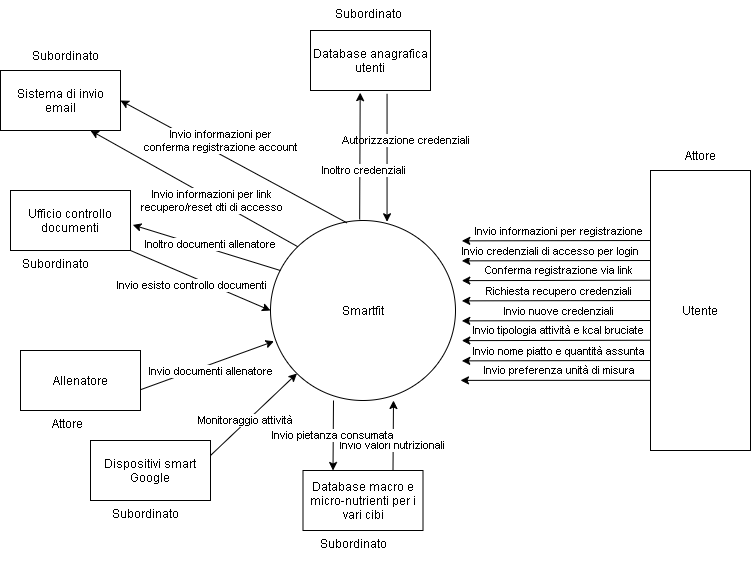
\includegraphics[width=175mm]{Diagramma di contesto.png}
      \section{Analisi dei componenti}
      Nel precedente capitolo è stata presentata l'architettura in termini di componenti esterni al sistema e come il sistema si interfaccia con essi. Ora, sempre sulla base dei
      requisiti dei precedenti documenti, si andrà invece a presentare l’architettura in termini dei componenti interni al sistema.Verranno identificati i vari componenti. Per ogni
      componente, oltre alla motivazione per la quale si è identificato tale componente, verrà descritto il suo scopo, il livello di coesione e ogni interfaccia fornita e richiesta.
      Verrà poi illustrato il diagramma dei componenti in cui si potrà vedere come i vari componenti interagiscono tra loro.\\


      {\Large\textbf{Gestione autenticazione}}\\

      \underline{Motivazione.} Dato il \textbf{RF3}, l’autenticazione dell’utente all’app avviene tramite username (o email) e password. Le credenziali di accesso sono salvate in un
      database esterno come descritto nell’ultimo punto del primo documento (back-end). Per questo scopo è stato identificato un componente \textbf{Gestione autenticazione} che si
      interfaccerà quindi con il sistema database anagrafica utenti che come detto è un servizio esterno. In particolare, il suddetto componente gestisce la procedura di login
      dell’utente munito di account, consentendo anche di inviare la richiesta di recupero password o username, anche questa descritta dal \textbf{RF3}.\\

      \textbf{Coesione:}livello \textbf{7} -funzionale.\\

      \underline{Spiegazione:} Il componente gestisce la funzionalità di autenticazione dell’utente munito di account all’interno dell’app, interfacciandosi con il database esterno.
      Gestisce inoltre la funzionalità di recupero credenziali.\\

      \underline{Descrizione:} il componente si occupa della funzionalità di autenticazione tramite le credenziali di accesso. Include una pagina per il login dell’utente in cui
      vengono richieste le credenziali. Si interfaccia poi con il database anagrafica esterno per l’autenticazione e da questo richiede anche la conferma per permettere o negare 
      l’accesso all’app. Il componente include anche la funzionalità di recupero password e/o username nel caso in cui l’utente se li fosse dimenticati. Si interfaccerà quindi anche
      con il sistema esterno di invio email.\\

      \underline{Interfaccia richiesta} – Credenziali. Le credenziali includono email, password e username. Sono richieste all’utente per la convalida sul sistema di autenticazione che fa
      riferimento a un database esterno.\\

      \underline{Interfaccia richiesta} – Conferma autenticazione. La convalida delle credenziali include la conferma o il rifiuto delle stesse, inclusi eventuali errori per utente inesistente. La
      conferma delle credenziali viene richiesta al sistema database anagrafica utenti (esterno), che permetterà o rifiuterà l’accesso all’app.\\

      \underline{Interfaccia fornita} – Credenziali utente. Le credenziali vengono fornite per un’altra interfaccia che procederà con l’autenticazione.\\

      \underline{Interfaccia fornita} – Informazioni email recupero password/username. Se l’utente richiede di reimpostare la password e/o lo username in caso se li fosse dimenticati, ci si
      affida al sistema esterno di invio email per l’invio dell'email contenente il link per tale operazione. Questa interfaccia fornirà quindi il destinatario, l’oggetto e il corpo
      della mail.\\


      {\Large\textbf{Gestione registrazione}}\\

      \underline{Motivazione.} Dato il \textbf{RF2}, al primo accesso l’utente deve creare un account. È stato quindi identificato un componente \textbf{Gestione registrazione} che si
      interfaccerà con il database esterno, già descritto nel componente Gestione autenticazione. In particolare, il componente gestisce la registrazione dell’utente interfacciandosi
      con il database esterno di anagrafica utenti.\\

      \textbf{Coesione:} livello \textbf{7} - funzionale.\\

      \underline{Spiegazione:} Il componente gestisce la funzionalità di creazione di un nuovo account da parte dell’utente al primo avvio dell’app, interfacciandosi con il database
      esterno. Si interfaccia inoltre con il sistema di invio email per l’invio della conferma di registrazione account.\\

      \underline{Descrizione:} Il componente quindi richiede le informazioni necessarie alla creazione di un nuovo account e poi si interfaccerà con il database per controllare che un
      account con lo stesso username e/o email non esista già. Questo componente, inoltre, dovrà interfacciarsi anche con un altro sistema esterno, ovvero il sistema per inviare email;
      a quest’ultimo il sistema deve inviare le informazioni necessarie (indirizzo email, oggetto e link per la conferma) per poter inviare la email che permetterà poi all’utente di
      confermare la creazione del nuovo account.\\

      \underline{Interfaccia richiesta} – Informazioni utente. Le informazioni includono: nome, cognome, data di nascita, peso, altezza, sesso e la preferenza sull'unità di misura
      (kg/m o lb/ft) per le conversioni delle misurazioni all'interno dell'app.\\

      \underline{Interfaccia richiesta} – Credenziali. Le credenziali includono email, password e username. Sono richieste all’utente per poterle poi inoltrare sul sistema di
      registrazione che fa riferimento a un database esterno.\\

      \underline{Interfaccia richiesta} – Verifica disponibilità. La conferma della disponibilità viene ricevuta da un’altra interfaccia dopo aver inviato a quest’ultima le
      credenziali. L’informazione è necessaria per gestire casi come la registrazione con credenziali già utilizzate per un altro account.\\

      \underline{Interfaccia richiesta} – Documenti allenatore. Per quanto riguarda la registrazione di un utente come allenatore è richiesto all'utente di inviare i documenti
      necessari a comprovare tale professione.\\

      \underline{Interfaccia fornita} - Documenti allenatore. I documenti di un allenatore vengono messi a disposizione per un'altra interfaccia che si occuperà della successiva
      convalida.\\

      \underline{Interfaccia fornita} – Credenziali utente. Le credenziali immesse dall’utente vengono messe a disposizione per essere poi inviate da un’altra interfaccia al sistema di 
      autenticazione.\\

      \underline{Interfaccia fornita} – Informazioni email verifica registrazione. Si mettono a disposizione le informazioni necessarie per l’invio di un’email contenente il link per
      la conferma della registrazione dell’account. L’interfaccia metterà quindi a disposizione il destinatario, l’oggetto e il corpo della email da inviare.\\


      {\Large\textbf{Modifica profilo utente}}\\

      \underline{Motivazione:} Dato il \textbf{RF11}, l’utente può modificare i propri dati personali e biometrici. Può anche inviare la richiesta per diventare allenatore inserendo i
      documenti necessari. È stato quindi identificato un componente \textbf{Modifica profilo utente}. In particolare, il componente permette all'utente di inserire i nuovi dati (personali e
      biometrici) e i documenti in caso l'utente volesse diventare un allenatore. Il componente si interfaccerà inoltre con l'interfaccia del database per il salvataggio dei nuovi
      dati dell'utente e con quella per l'invio delle email per l'invio del link per il reset dei dati personali.\\

      \textbf{Coesione:} livello \textbf{6} - informazionale.\\

      \underline{Spiegazione:} Il componente gestisce la modifica delle informazioni che l’utente aveva precedentemente inserito al momento della registrazione. Quindi non è
      funzionale dato che non va a svolgere una singola funzione, ma più funzioni che comunque sono collegate fra loro dato che tutte riguardano la modifica dei dati personali e si
      interfacciano con il database esterno.\\

      \underline{Descrizione:} Questo componente richiede quindi i nuovi dati utente (personali o biometrici) e anche i documenti per diventare allenatore i quali vengono poi inviati
      al sistema esterno di validazione come già descritto per il componente Gestione registrazione. Dato che va a modificare i dati dell’utente, questo deve interfacciarsi con il
      database per aggiornare i dati e ovviamente controllare la disponibilità nel caso in cui si vada a cambiare username e/o email. Va anche a interfacciarsi con il sistema esterno
      di controllo documenti nel caso in cui l’utente voglia diventare allenatore. Infine, dovrà interfacciarsi con il sistema esterno per l’invio di email per l’invio all’utente del
      link per il reset di password e/o email.\\

      \underline{Interfaccia richiesta} - Nuovi dati biometrici. Viene richiesto all’utente di inserire i nuovi dati biometrici. Per dati biometrici si intendono le informazioni
      dell’utente che venivano inseriti anche nel componente di gestione della registrazione, quindi: nome, cognome, data di nascita, peso, altezza, sesso e la preferenza sull'unità di
      misura (kg/m o lb/ft) per le conversioni delle misurazioni all'interno dell'app.\\

      \underline{Interfaccia richiesta} – Nuovi dati personali. Viene richiesto all’utente di inserire i nuovi dati personali, ovvero la nuova password, email o lo username.\\

      \underline{Interfaccia richiesta} – Documenti allenatore. Per quanto riguarda la registrazione di un utente come allenatore è richiesto all'utente di inviare i documenti necessari
      a comprovare tale professione.\\

      \underline{Interfaccia richiesta} – Verifica disponibilità. La conferma della disponibilità viene ricevuta da un’altra interfaccia dopo aver inviato a quest’ultima le credenziali.
      L’informazione è necessaria per gestire il caso in cui si cerca di cambiare la email con una già collegata con un altro account.\\

      \underline{Interfaccia fornita} – Documenti allenatore. I documenti di un allenatore vengono messi a disposizione per un'altra interfaccia che si occuperà della successiva
      convalida.\\

      \underline{Interfaccia fornita} – Informazioni email recupero password/username. Se l’utente richiede di reimpostare la password e/o lo username in caso se li fosse dimenticati,
      ci si affida al sistema esterno di invio email per l’invio dell'email contenente il link per tale operazione. Questa interfaccia fornirà quindi il destinatario, l’oggetto e il
      corpo della mail.\\

      \underline{Interfaccia fornita} – Modifica dati personali. Vengono messi a disposizione per l’interfaccia di gestione anagrafica utenti i nuovi dati da inserire di cui l’utente
      ha richiesto la modifica e inserito i nuovi.\\


      {\Large\textbf{Gestione allievi}}\\

      \underline{Motivazione:} Dati i \textbf{RF13, RF14, RF15 e RF16}, un allenatore può cercare e aggiungere allievi e ad essi può inviare schede di allenamento e di alimentazione. Un
      allenatore può inoltre visionare l’andamento di un suo allievo. È stato quindi identificato un componente \textbf{Gestione allievi}. In particolare, questo componente permette all’
      allenatore di cercare ed aggiungere allievi, creare delle schede di allenamento e di alimentazione che da inviare loro e infine prendere visione dell’andamento di un allievo.\\

      \textbf{Coesione:} livello \textbf{6} - informazionale.\\

      \underline{Spiegazione:} il componente contiene tutte e sole le funzioni che vedono l’interazione allenatore-cliente dalla parte dell’allenatore. Si poteva dividere facilmente
      in due componenti di livello funzionale, però si è preferito sacrificare un livello per rendere il diagramma stesso più leggibile altrimenti si andavano a creare forse un po’ 
      troppi componenti che dovevano svolgere funzioni molto piccole.\\

      \underline{Descrizione:} Il componente permette all’allenatore di cercare un utente tramite email o username e inviargli una richiesta per associarsi ad esso. Dovrà quindi
      interfacciarsi con l’interfaccia dell’anagrafica utenti per poter trovare un utente. Permette inoltre di creare e successivamente inviare schede di alimentazione e di
      allenamento; si ricorda che si può inviare massimo una scheda per tipo ad ogni allievo. L’allenatore può anche avere tutte le informazioni sull’andamento di un suo allievo,
      ovvero le kcal consumate e con che attività fisica, nonché le kcal assunte e con che pasti.\\

      \underline{Interfaccia richiesta} – Visualizzazione andamento allievo. L’andamento allievo è la cronologia di un utente che include le kcal assunte e bruciate con le varie
      attività fisiche e i pasti consumati.\\

      \underline{Interfaccia richiesta} – Conferma associazione. L’allenatore può solo inviare una richiesta di associazione quindi questa deve essere confermata dall’utente per poter
      diventare un suo allievo. Questa interfaccia dovrà quindi interfacciarsi con il l’utente per prelevare il risultato della richiesta.\\

      \underline{Interfaccia richiesta} – Conferma presenza utente. Questa interfaccia va a richiedere il risultato della ricerca di un utente al sistema di gestione account.\\

      \underline{Interfaccia fornita} – Scheda di allenamento. L’allenatore può inviare ai propri allievi le varie schede di allenamento (massimo una per ognuno) dopo averla creata.\\

      \underline{Interfaccia fornita} – Aggiunta allievo. L’allenatore invia la richiesta di associazione a un utente, quest’ultimo potrà poi accettarla e diventare suo allievo o
      rifiutarla.\\

      \underline{Interfaccia fornita} – Scheda di alimentazione. L’allenatore può inviare ai propri allievi le varie schede di allenamento (massimo una per ognuno) dopo averla creata.\\

      \underline{Interfaccia fornita} – Ricerca utente. La ricerca fornisce l’email o lo username di un utente per permettere al sistema di gestione utenti di ricercarlo.\\


      {\Large\textbf{Gestione allenatore e schede}}\\

      \underline{Motivazione:} Dati i \textbf{RF9, RF10, RF14 e RF15,} l’utente può accettare o rifiutare la richiesta di associazione da parte di un allenatore. Può visualizzare le
      schede di alimentazione e allenamento che il proprio allenatore gli ha inviato, ovvero come detto massimo una di alimentazione e massimo una di allenamento. È stato quindi
      identificato un componente \textbf{Gestione allenatore e schede}. In particolare, il componente si occupa della gestione dell’associazione tra allenatore e allievo, nonché della
      visualizzazione delle schede ricevute dal proprio allenatore e le informazioni dell’allenatore stesso.\\

      \textbf{Coesione:} livello \textbf{6} - Informazionale.\\

      \underline{Spiegazione:} anche in questo caso il componente contiene tutte e sole le funzioni che vedono l’interazione allenatore-cliente però dalla parte dell’utente. Come
      anche per il componente di gestione allievi, si poteva dividere facilmente in due componenti di livello funzionale, però si è preferito sacrificare un livello per rendere il
      diagramma stesso più leggibile.\\

      \underline{Descrizione:} Il componente permette all’allievo di accettare o rifiutare la richiesta di associazione da parte di un allenatore. Permette inoltre di ricevere le
      schede di alimentazione e allenamento dal proprio allenatore e quindi di visualizzarle. Infine, permette all’utente di visualizzare le informazioni del proprio utente (nome,
      età, ecc.). Dal momento che un utente può avere contemporaneamente solo un allenatore associato ad esso, come specificato nei requisiti funzionali del primo documento di
      specifiche del progetto, il componente permette l’eliminazione/sostituzione del proprio allenatore con un altro accettando una nuova richiesta di associazione.\\

      \underline{Interfaccia richiesta} –  Scheda di allenamento. L’utente riceve la scheda di allenamento dal proprio allenatore.\\

      \underline{Interfaccia richiesta} – Scheda di alimentazione. L’utente riceve la scheda di allenamento dal proprio allenatore.\\

      \underline{Interfaccia richiesta} – Aggiunta allievo. L’utente riceve le richieste di associazione dai vari allenatori.\\

      \underline{Interfaccia fornita} –  Conferma associazione. L’utente può decidere se accettare o rifiutare l’associazione richiesta da un particolare allenatore.\\

      \underline{Interfaccia fornita }– Visualizzazione allenatore. Le informazioni di un allenatore includono le varie informazioni biometriche che l’allenatore ha inserito\\
      nell’applicazione al momento della registrazione (o successivamente se le ha cambiate dalla gestione profilo). Includono quindi nome, cognome, età, peso e altezza e sesso.\\

      \underline{Interfaccia fornita} – Visualizzazione scheda personalizzata. L’utente può visualizzare la scheda (massimo una di alimentazione e una di allenamento) che il proprio
      allenatore gli ha inviato.\\


      {\Large\textbf{Andamento utente}}\\

      \underline{Motivazione:} Dato il \textbf{RF6}, l’utente può visualizzare la propria cronologia di calorie assunte e bruciate, nonché le attività fisiche svolte e i pasti assunti. È
      stato quindi identificato un componente \textbf{Andamento utente} che prelevando i dati riguardanti dieta e allenamento tiene una cronologia con kcal bruciate e assunte, gli allenamenti
      fatti e i pasti assunti per 14 giorni come da requisito nel documento delle specifiche del progetto.\\

      \textbf{Coesione:} livello \textbf{7} – funzionale.\\

      \underline{Spiegazione:} il componente gestisce la funzionalità di visualizzazione cronologia allenamento e dieta da parte di un determinato utente.\\

      \underline{Descrizione:} il componente preleva i dati sugli allenamenti e pasti consumati dai relativi sistemi di gestione per poi creare una cronologia di 14 giorni su tutte
      le informazioni fornite di un determinato utente. Fornisce sia la funzione di visualizzazione della cronologia di un determinato utente da parte dell’utente stesso sia dal
      proprio allenatore.\\

      \underline{Interfaccia richiesta} – Pasti consumati. Il componente richiede i pasti assunti dall’utente con i relativi valori nutrizionali associati.\\

      \underline{Interfaccia richiesta} – Attività svolte. Il componente richiede le attività fisiche svolte dall’utente con i relativi consumi di kcal.\\

      \underline{Interfaccia fornita} – Visualizzazione cronologia dieta e attività. Il componente mette a disposizione dell’utente la propria cronologia di pasti assunti e attività
      svolte con i relativi valori nutrizionali, kcal assunte e bruciate.\\

      \underline{Interfaccia fornita} – Visualizzazione andamento allievo. Il componente mette a disposizione dell’allenatore la cronologia, di un suo allievo, di pasti assunti e
      attività svolte con i relativi valori nutrizionali, calorie assunte e bruciate.\\
      \\
      \\


      {\Large\textbf{Gestione dieta}}\\

      \underline{Motivazione:} Dato il \textbf{RF5} e il \textbf{RF7}, l’utente può aggiungere e rimuovere pasti e visualizzare il riepilogo giornaliero delle Kcal e dei micro e macronutrienti assunti.
      È stato individuato un componente \textbf{Gestione dieta}. In particolare, il componente ricevendo le informazioni sui pasti consumati va a calcolare i valori nutrizionali
      interfacciandosi con un altro componente e poi mette a disposizione il riepilogo dei pasti assunti.\\

      \textbf{Coesione:} livello \textbf{7} - funzionale.\\

      \underline{Spiegazione:} Il componente è necessario per la funzione di inserimento dei pasti dell’utente che permette l’esistenza della funzione di visualizzazione del bilancio
      giornaliero di kcal e di micro e macronutrienti.\\

      \underline{Descrizione:} il componente riceve le informazioni sul pasto consumato dall’utente e interfacciandosi con l’interfaccia del database nutrienti permette di
      visualizzare il riepilogo giornaliero delle calorie e dei micro e macronutrienti assunti dall’utente. Viene fornita sia un’interfaccia per il riepilogo giornaliero sia un
      interfaccia con i vari pasti assunti.\\

      \underline{Interfaccia richiesta} – Pasto. Viene richiesto all’utente di inserire la pietanza consumata e la relativa quantità.\\

      \underline{Interfaccia richiesta} – Macro e micro nutrienti. Dopo aver inviato le informazioni riguardanti il pasto consumato dall’utente si richiedono i valori nutrizionali
      associati, questi verranno forniti da un altro componente.\\

      \underline{Interfaccia fornita} – Riepilogo pasti giornalieri. Il componente fornisce il riepilogo giornalieri di pasti assunti con i relativi valori nutrizionali e kcal
      assunte.\\

      \underline{Interfaccia fornita} – Pasti consumati. Il componente fornisce tutti i vari pasti consumati dall’utente con quantità, valori nutrizionali e kcal assunte.\\
 
      \underline{Interfaccia fornita} – Pietanza. Il componente mette a disposizione le varie singole pietanze consumate dall’utente per il calcolo dei valori nutrizionali da parte
      di un altro componente.\\


      {\Large\textbf{Gestione allenamento}}\\

      \underline{Motivazione:} Per il \textbf{RF7} l’utente può aggiungere un’attività fisica svolta con il le relative kcal bruciate. È stato individuato un componente
      \textbf{Gestione allenamento}.
      In particolare, il componente riceve le informazioni riguardanti l’allenamento e le mette a disposizione per gli altri componenti.\\

      \textbf{Coesione:} livello \textbf{7} - funzionale.\\

      \underline{Spiegazione:} Il componente è necessario per la funzione di inserimento delle attività svolte dall’utente.\\

      \underline{Descrizione:} il componente permette di inserire le varie attività svolte da parte dell’utente, le quali possono provenire sia dall’utente stesso inserendole in una
      text-box o anche dai dispositivi smart di Google come specificato nei requisiti nel documento delle specifiche del progetto.\\

      \underline{Interfaccia richiesta} – Attività. Il componente richiede le attività svolte da parte dell’utente. Queste come detto possono provenire da varie fonti, nello
      specifico dai dispositivi smart Google o dall’inserimento manuale da parte dell’utente.\\

      \underline{Interfaccia fornita} - Attività svolte. Il componente mette a disposizione ogni attività svolta dall’utente con le relative kcal bruciate per la cronologia
      dell’utente affidata ad un altro componente.\\


      {\Large\textbf{Database nutrienti}}\\

      \underline{Motivazione:} Dato il \textbf{RF7}, quando si aggiunge un pasto assunto (di cui si occupa il componente Gestione dieta) vengono automaticamente calcolati i corrispondenti
      valori nutrizionali. Come specificato dal \textbf{RF7} e nella sezione backend del documento delle specifiche del progetto, per questo calcolo ci si appoggia a un database esterno che
      contiene associazioni tra pietanze e valori nutrizionali. Per interfacciarsi con questo database esterno è stato identificato un componente \textbf{Database nutrienti}. In particolare,
      questo componente richiede le informazioni della pietanza (nome e quantità) per poi generare una query al database e riportare i risultati.\\

      \textbf{Coesione:} livello \textbf{7} - funzionale.\\

      \underline{Spiegazione:} Il componente gestisce la funzionalità di calcolo automatico dei valori nutritivi delle pietanze aggiunte dall’utente.\\

      \underline{Descrizione:} Il componente dopo aver ricevuto le informazioni riguardanti una pietanza assunta dall’utente con la relativa quantità, genera una query che poi
      inoltrerà al sistema database esterno per il calcolo dei valori nutrizionali e poi fornire tali dati alla gestione dieta dell’utente.\\

      \underline{Interfaccia richiesta} – Pietanza. Vengono richieste le informazioni sulla pietanza assunta dall’utente (nome e quantità).\\

      \underline{Interfaccia richiesta} – Risposta. Dopo aver inviato la query al database esterno, il componente aspetta la risposta per poi comunicarla agli altri componenti che
      hanno generato la richiesta.\\

      \underline{Interfaccia fornita} – Macro e micronutrienti. Dopo aver generato e inoltrato la query al database esterno, il componente fornisce i vari valori funzionali della
      pietanza assunta dall’utente.\\

      \underline{Interfaccia fornita} – Query. Il componente genera ed inoltra una query al database esterno, nello specifico la query in questione è un selezionamento alla base
      della pietanza che è stata comunicata da un altro componente.\\


      {\Large\textbf{Database anagrafica utenti}}\\

      \underline{Motivazione:} Dati i \textbf{RF2} e \textbf{RF3}, l’utente necessita di un account per poter utilizzare questa app. L’account viene creato con un indirizzo e-mail e altre informazioni
      già specificate per i componenti corrispondenti. Queste informazioni vengono salvate in un database, nello specifico in un database esterno come scritto nella sezione backend del
      documento delle specifiche del progetto. Inoltre, anche per il cambiamento delle credenziali degli utenti specificato nel \textbf{RF11} si devono inviare le nuove credenziali al database.
      Per interfacciarsi con il suddetto database esterno è stato identificato un componente \textbf{Database anagrafica utenti}. In particolare, questo componente riceve le informazioni
      necessarie alla registrazione o all’accesso  o le nuove credenziali per la modifica e genera una query al database, inviando poi la conferma che la procedura sia andata a buon
      fine.\\

      \textbf{Coesione:} livello \textbf{7} - funzionale.\\

      \underline{Spiegazione:} Il componente è necessario per entrambe le funzionalità di autenticazione e registrazione andando a salvare e richiedere informazioni al database esterno
      contenente tutte le credenziali degli utenti. Inoltre, il database è anche necessario per la funzionalità di recupero credenziali utente che viene eseguita dal componente
      Modifica profilo utente.\\

      \underline{Descrizione:} il componente gestisce l’interfaccia con il database, il quale come detto è un sistema esterno come specificato nella sezione backend del documento
      delle specifiche progetto. Riceverà quindi le credenziali dell’utente, che esse siano per l’autenticazione, per la registrazione di un account o per modifica di esse. Potrà anche
      ricevere semplicemente email o username di un utente per cercarlo all’interno del sistema esterno. Il componente procederà quindi con la creazione e inoltro della query al
      database esterno per poi ricevere la risposta da parte del database, che sia solo una conferma di avvenuta modifica/inserimento o per i dati risultato della query.\\

      \underline{Interfaccia richiesta} – Credenziali utente. Il componente chiede le credenziali dell’utente, che possono essere username email e password in caso di registrazione
      oppure solo password e email o username per l’autenticazione.\\

      \underline{Interfaccia richiesta} – Ricerca utente. Le informazioni necessarie per la ricerca di un utente includono solo l’indirizzo email e/o lo username.\\

      \underline{Interfaccia richiesta} – Risposta. Una volta inoltrata la query al database esterno il componente aspetta la risposta di esso per poterla comunicare agli altri
      componenti.\\

      \underline{Interfaccia richiesta} – Modifica dati personali. Il componente richiede all’utente di inserire i dati di cui ha richiesto la modifica.\\

      \underline{Interfaccia fornita} – Conferma autenticazione. Il componente fornisce la conferma che un’autenticazione sia andata a buon fine.\\

      \underline{Interfaccia fornita} – Conferma presenza utente. Il componente fornisce i dati necessari alla comunicazione con un determinato utente in caso lo avesse trovato nel
      database esterno.\\

      \underline{Interfaccia fornita} – Verifica disponibilità. Il componente, nel caso in cui si cerchi di creare un account con indirizzo email o uno username già utilizzato,
      comunica all’utente l’impossibilità di creare un account con tali dati.\\

      \underline{Interfaccia fornita} – Query. La query dipende dalla funzionalità che si è richiesta al componente, può essere che sia un inserimento nel caso della registrazione o
      modifica dati oppure un selezionamento nel caso di autenticazione o ricerca utente.\\



      {\Large\textbf{Controllo documenti}}\\

      \underline{Motivazione:} Dato il \textbf{RF2}, un allenatore per registrarsi come tale necessita di caricare i propri documenti nell’app, i quali poi verranno inviati a un
      ufficio esterno per la verifica e una volta verificati avrà a disposizione le funzionalità per poter lavorare. Nel \textbf{RF11} viene anche specificato che anche un utente base può
      diventare allenatore se invia i propri documenti necessari anche dopo la registrazione, ovvero dalla modifica profilo utente, con la stessa procedura fatta nella registrazione.
      Per interfacciarsi con il sopracitato ufficio è stato individuato un componente \textbf{Controllo documenti}. In particolare, questo componente riceve i documenti dell’allenatore e li
      invia all’ufficio predisposto per la validazione.\\

      \textbf{Coesione:} livello \textbf{7} - funzionale\\

      \underline{Spiegazione:} Il componente è necessario per la funzione di registrazione all’app di un allenatore.\\

      \underline{Descrizione:} il componente una volta ricevuti i documenti necessari all’allenatore procede con l’invio degli stessi all’ufficio preposto. Sarà inoltre necessario un
      flusso di informazioni dall’ufficio verso il componente per il requisito funzionale nel documento dei requisiti del progetto in cui viene specificato che ci deve anche essere una
      notifica in-app, di cui si occuperà quindi questa interfaccia.\\

      \underline{Interfaccia richiesta} – Documenti allenatore. L’interfaccia richiede i documenti da validare all’utente.\\

      \underline{Interfaccia richiesta} – Validità documenti. Dopo aver inviato i documenti all’ufficio di validazione, riceverà la risposta della convalida, che potrà essere
      l’accettazione o il rifiuto di tali documenti.\\

      \underline{Interfaccia fornita} – Mostra documenti da validare. L’interfaccia metterà a disposizione i documenti dell’allenatore verso le interfacce del sistema esterno 
      dell’ufficio di convalida degli stessi.\\


      {\Large\textbf{Invio email}}\\

      \underline{Motivazione:} Dato il \textbf{RF2} per la conferma della registrazione di un account è necessario confermare la registrazione con un link inviato via email, e lo stesso vale
      per il \textbf{RF3} e il \textbf{RF11} in cui viene inviata una email per il reset della password e/o username. Per l’invio delle email agli utenti viene utilizzato un sistema esterno come
      specificato nella sezione backend del documento delle specifiche del progetto. È stato quindi individuato il componente \textbf{Invio email}. In particolare, il componente dopo aver
      ricevuto le informazioni necessarie, si interfaccerà con il sistema esterno per inviare la email richiesta.\\

      \textbf{Coesione:} livello \textbf{7} - funzionale\\

      \underline{Spiegazione:} Il componente è necessario per interfacciarsi con il sistema esterno di invio email che permette l’invio della email per la conferma della registrazione
      e per il reset della password.\\

      \underline{Descrizione:} il componente viene fornito delle informazioni necessarie per l’invio di una email, quindi email dell’utente, oggetto della email e il contenuto del
      messaggio. Il contenuto del messaggio dipende da che tipo di email si vuole inviare, nel caso della conferma di registrazione sarà un link per confermare la procedura. Nel caso
      in cui si voglia inviare la email per il reset della password o dello username il contenuto della email sarà un altro link che porterà alla pagina di reset. Il componente si
      interfaccerà poi con il sistema esterno di invio email a cui invierà le varie informazioni.\\

      \underline{Interfaccia richiesta} – Informazioni email recupero password/username. Il componente richiede le informazioni necessarie per l’invio della email di recupero
      password e/o username. In particolare, dovrà ricevere la email del destinatario, l’oggetto e il corpo della mail che sarà quindi il link che porterà alla pagina di reset di
      tali dati.\\

      \underline{Interfaccia richiesta} – Informazioni email verifica registrazione. Il componente richiede le informazioni necessarie per l’invio della email di conferma di
      registrazione di un nuovo account. In particolare, dovrà ricevere la email del destinatario, l’oggetto e il corpo della mail che sarà quindi il link che porterà alla pagina di
      conferma e verifica email.\\

      \underline{Interfaccia fornita} – Email. L’interfaccia, dopo aver ricevuto le informazioni necessarie, invia tutte queste informazioni pronte per essere inviate al sistema
      esterno di invio email che procederà direttamente all’invio delle stesse.\\

      \newpage
      \section{Tabella riassuntiva dei livelli di coesione dei componenti}
      \begin{center}
            \begin{tabular}{|p{3 cm}|c|c|c|c|c|c|c|}
                  \hline
                  Componenti/Livello di coesione & 1 casuale & 2 logica & 3 temporale & 4 procedurale & 5 comunicazionale & 6 informazionale & 7 funzionale\\
                  \hline
                  Gestione autenticazione&&&&&&&x\\
                  \hline
                  Gestione registrazione&&&&&&&x\\
                  \hline
                  Modifica profilo utente&&&&&&x&\\
                  \hline
                  Gestione allievi&&&&&&x&\\
                  \hline
                  Gestione allenatore e schede&&&&&&x&\\
                  \hline
                  Andamento utente&&&&&&&x\\
                  \hline
                  Gestione dieta&&&&&&&x\\
                  \hline
                  Gestione allenamento&&&&&&&x\\
                  \hline
                  Database nutrienti&&&&&&&x\\
                  \hline
                  Database anagrafica utenti&&&&&&&x\\
                  \hline
                  Controllo documenti&&&&&&&x\\
                  \hline
                  Invio email&&&&&&&x\\
                  \hline
            \end{tabular}
      \end{center}
      \section{Diagramma dei componenti e BPMN}
      \begin{center}
            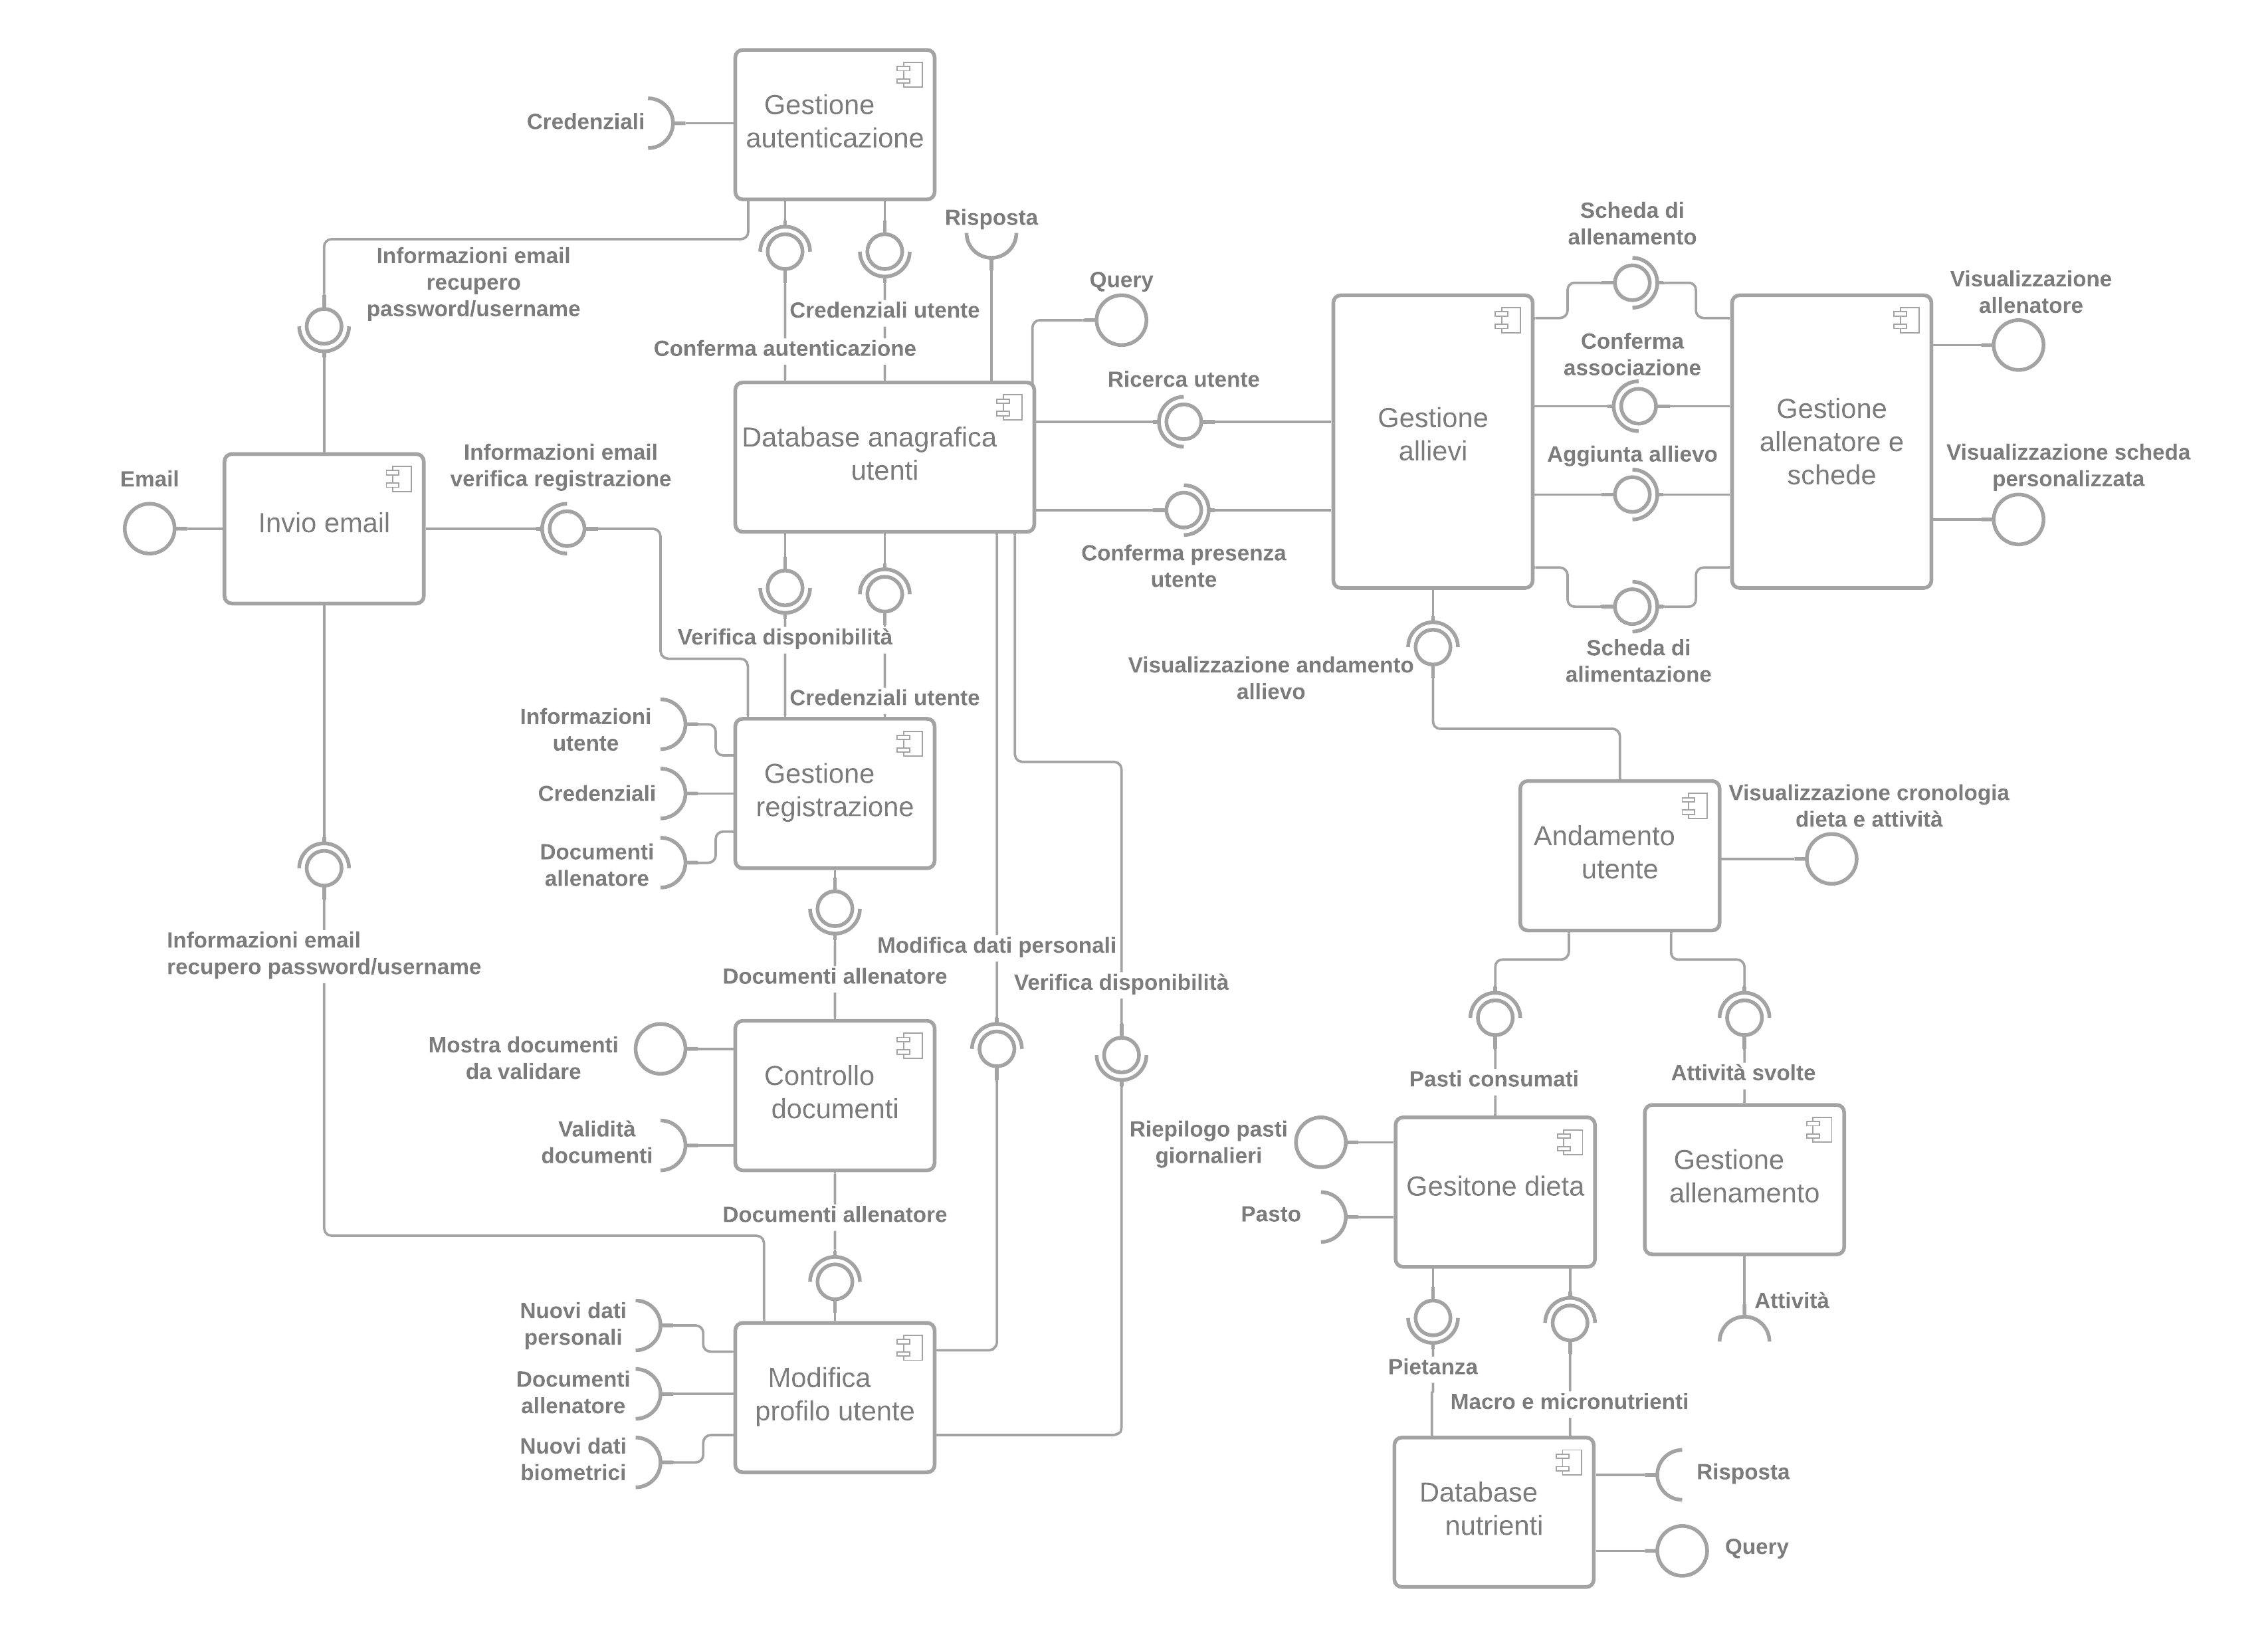
\includegraphics[width=200mm]{Component diagram.png}
      \end{center}
      \begin{center}
            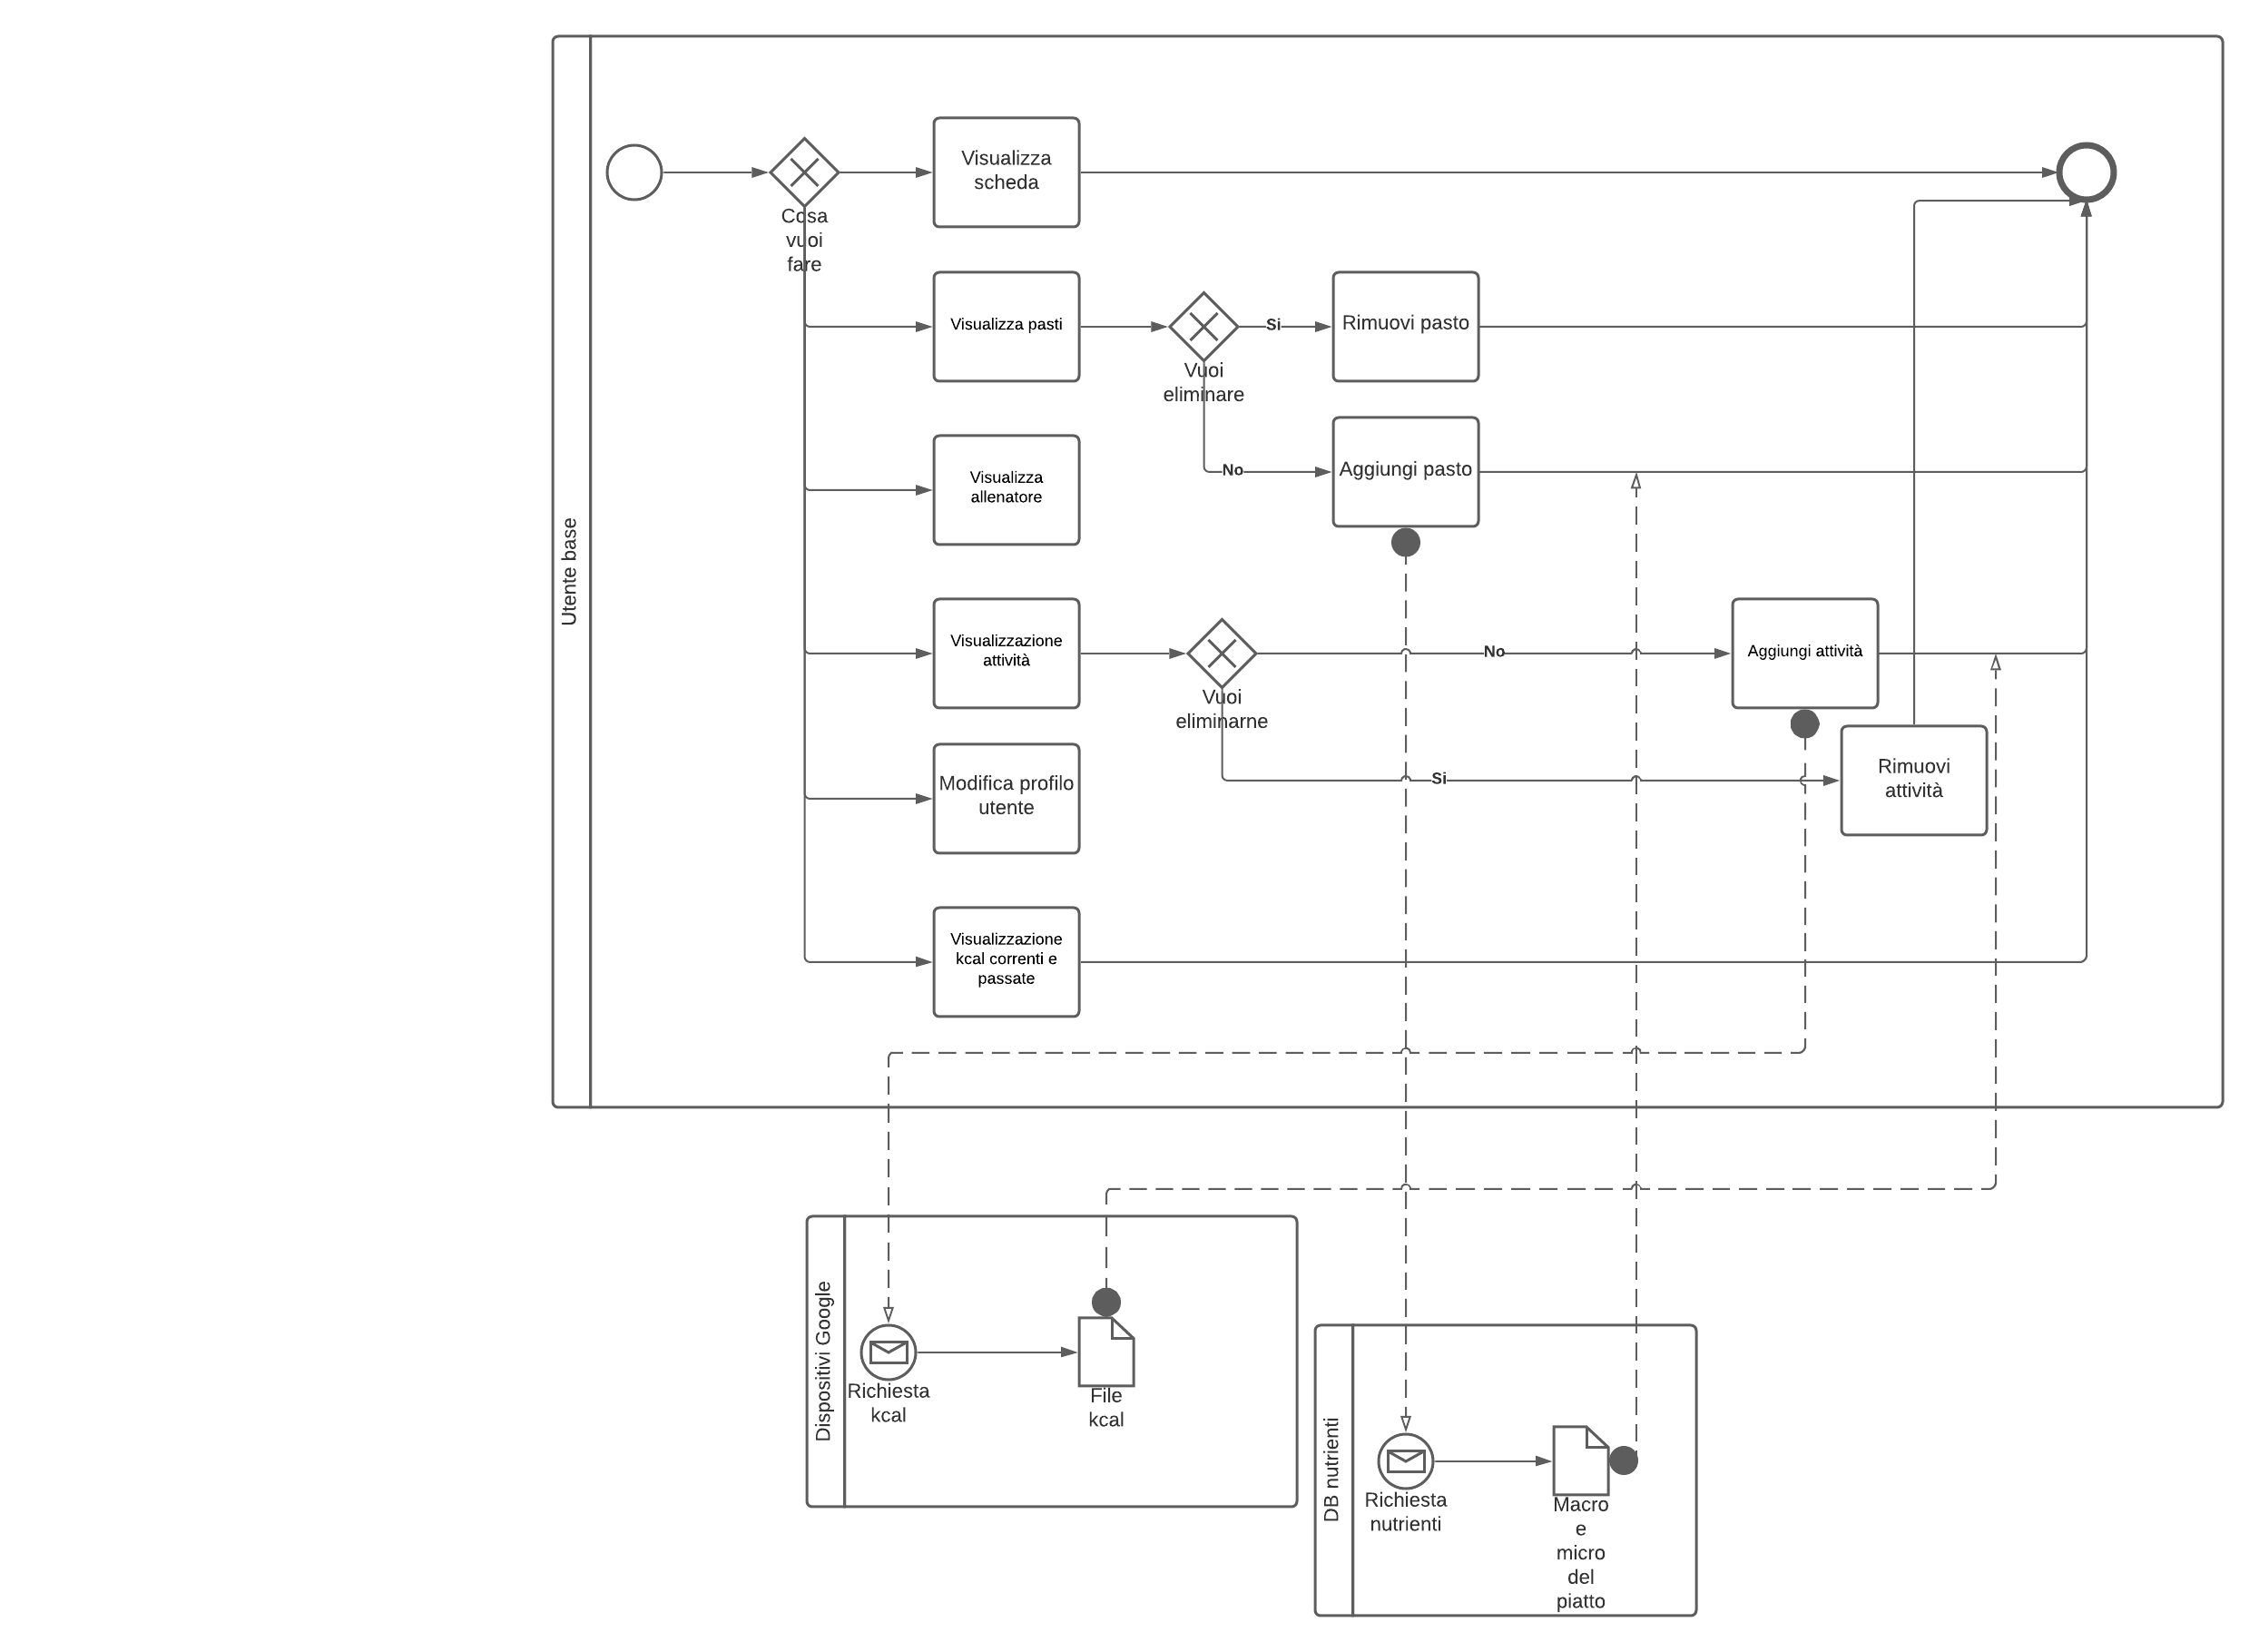
\includegraphics[width=200mm]{BPMN1.png}
      \end{center}
      \begin{center}
            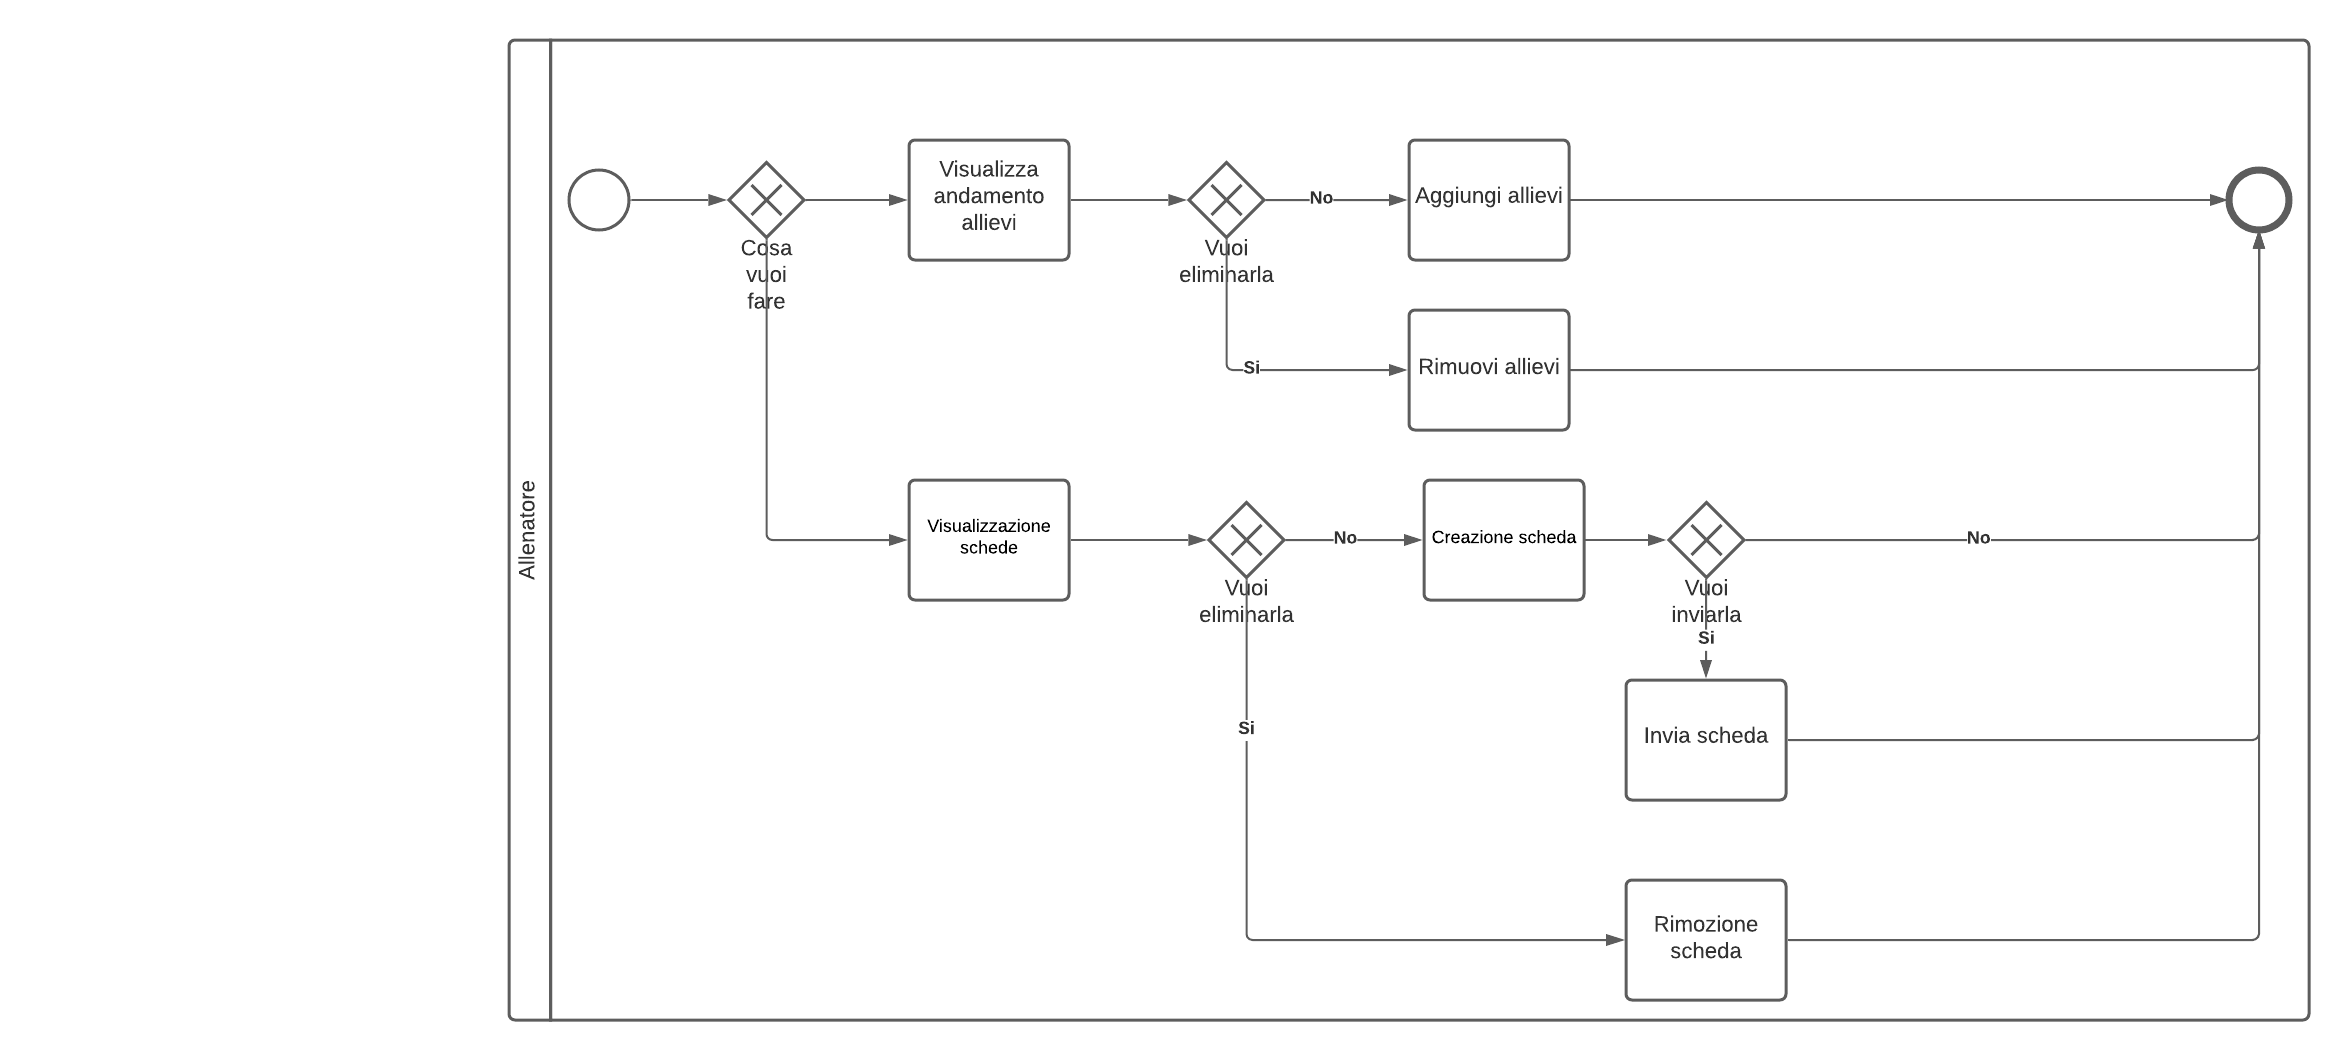
\includegraphics[width=200mm]{BPMN2.png}
      \end{center}     
\end{document}